% 4 Data

% 4.1 Data Sources and Sample Period
%   4.1.1 CRSP/Compustat via WRDS – stock returns, volume, market equity, bid–ask spreads
%   4.1.2 Fama–French factor series (MKT, SMB, HML, RMW, CMA) from Kenneth French’s library
%   4.1.3 Liquidity proxies from CRSP daily files (turnover, Amihud ILLQ, zero‐trade days)
%   4.1.4 Sentiment index (STV) from Ung et al. (2024) supplemental data
%   4.1.5 Sector classification via Compustat’s comp.company (SIC/NAICS codes)
%   Table 4.1: Data sources, sample periods, update frequencies

% 4.2 Sample Selection and Coverage
%   4.2.1 Chronology: January 1990–December 2018 (pre-COVID)
%   4.2.2 Stock inclusion criteria: PERMNO universe, liquidity thresholds, delisting handling
%   4.2.3 Survivorship bias mitigation (CRSP historical constituents)
%   4.2.4 Matching factor, liquidity and sentiment series to equity returns

% 4.3 Variable Construction
%   4.3.1 Monthly excess returns:  

%   (CRSP return minus 1-month T-bill)
%   4.3.2 Fama–French factors: construction and alignment with return data
%   4.3.3 Liquidity measures:
%     
% ∙
% ∙ Amihud illiquidity (ILLQ) formula and scaling
%     
% ∙
% ∙ Turnover, turnover volatility, zero-trade days, bid–ask spread
%     — cross-sectional ranking and standardization to [–1, 1]
%   4.3.4 Investor sentiment (STV): rolling‐window PCA on six Baker–Wurgler proxies; orthogonalization to business-cycle factors
%   4.3.5 Normalization and winsorization procedures

% 4.4 Sector Classification
%   4.4.1 Mapping PERMNO ↔ SIC/NAICS codes → GICS sectors
%   4.4.2 Aggregation to 10 major sectors
%   Table 4.2: Sector definitions and ticker counts by sector

% 4.5 Data Cleaning and Pre-processing
%   4.5.1 Treatment of missing observations (listwise deletion vs. interpolation)
%   4.5.2 Outlier handling: winsorization at 1st/99th percentiles
%   4.5.3 Lagging variables and alignment (e.g., sentiment(t–1), ILLQ(t))
%   4.5.4 Final panel construction: balanced vs. unbalanced tests

% 4.6 Descriptive Statistics and Preliminary Visualizations
%   4.6.1 Summary statistics for all variables (mean, SD, skew, kurtosis)
%   Table 4.3: Descriptive statistics of returns, factors, liquidity, sentiment
%   4.6.2 Histograms of ILLQ, turnover, sentiment index—assess distributional shape
%   Figure 4.1: Histogram grid of liquidity proxies and STV
%   4.6.3 Time‐series plots of aggregate liquidity and sentiment indices (1990–2018)
%   Figure 4.2: Overlay of monthly Amihud ILLQ and STV series
%   4.6.4 Cross‐variable correlation heatmap (factors vs. liquidity vs. sentiment)
%   Figure 4.3: Correlation matrix heatmap

% 4.7 Data Summary and Key Takeaways
%   4.7.1 Coverage and quality of main variables
%   4.7.2 Observed stylized facts (e.g., liquidity spikes in crises, sentiment cycles)
%   4.7.3 Implications for subsequent modeling chapters

% Placement of Figures/Tables

% Table 4.1 immediately after Section 4.1.

% Table 4.2 at the end of Section 4.4.

% Table 4.3 at the start of Section 4.6, before the histogram panel.

% Figure 4.1 and Figure 4.2 side by side (two-column layout) within Section 4.6.

% Figure 4.3 full-width heatmap at the end of Section 4.6.

\subsection{Data Sources and Sample Period}\label{sec:data_sources}

This study integrates equity, option, and macro-factor information from several well-established WRDS libraries. Daily common-share returns,risk free rate, market returns, share volume, shares outstanding, trade-conditioned prices, and intraday high/low quotes are drawn from the \emph{CRSP Daily Stock File} \cite{crsp_dsf}. Corporate identifiers (PERMNO) are matched to tickers, historical company names, and exchange codes table, ensuring that delisted and renamed firms remain in the final analysis. The initial CRSP extraction contains every ordinary common share listed on the NYSE,NYSE MKT, NASDAQ and Arca exchanges between 1998 and 2018. 

The returns of this dataset value weighted and is extracted without dividends.To mitigate microstructure noise, daily returns are discarded if any of the following conditions hold: (i) the absolute price is below \$1; (ii) share volume is missing; or (iii) CRSP marks the observation with a non-regular return code.

To filter out the stocks within the \emph{CRSP Daily Stock File}  that are not members of the SP500 index, the table is intersected with the historical \emph{S\&P 500 Constituents List} \cite{compstat}. The list provides the member entry  and member exit dates for every constituent since 1990. Merging the two datasets on PERMNO and calendar date yields a time-varying panel that includes each firm only during its actual index membership window, which eliminates survivorship bias arising from back-filling non-constituent observations. This means that companies that enters the S\&P500 is only included in their entry date onwards, while those that either went bankrupt, removed from the index or that got acquired after 2018 remains in the analysis. After intersecting with the S\&P500 membership file, the total number of companies remaining in the analysis is limited to 1063 unique firms that have belonged to the index at least once during the sample period. Each security contributes observations only for the days on which it is an official constituent, thereby mirroring the investable set faced by index-tracking portfolios (such as the publicly traded S\&P500 index) in real time.

Sector classification information is sourced from the \emph{Compustat North America} header table, which reports each firm's \texttt{gsector}—a two-digit sector code consistent with the Global Industry Classification Standard (GICS) \cite{compstat}. This differs from the other datasets, which primarily identify firms using the \texttt{permno} variable. Because CRSP and Compustat utilizes different primary keys, firm-level observations are linked via a CRSP-Compustat bridge table. This particular link enable one-to-one mappings between CRSP's PERMNO and Compustat's \textsc{gvkey}.Daily macro-risk factors are sourced from Kenneth French's library,also available from WRDS, providing the market excess return ($RF_{MKT}$), size ($SMB$), value ($HML$), profitability ($RMW$), investment ($CMA$), momentum ($UMD$) and the treasury rate ($RF$) \cite{ff_wrds}. These series are merged to the equity panel on the trading date.

Finally, index-level option activity is captured through \citeA{optionsmetrics}. Put and call trading volumes for each security identifier (\textsc{secid}) are aggregated to the daily level. The WRDS-supplied correspondence file maps each \textsc{secid} to its CRSP PERMNO over time. OptionMetrics coverage is less complete than CRSP coverage, particularly prior to 2000 when listed index options were thinly traded, or the data was not recorded properly. This could corrupt the dataset as both zero value and unavailable/corrupted call or put volume is registered in WRDS as 0.0. Nonetheless, a large portion of put-call pairs possess at least one non-missing put or call volume observation. For days in which one side of the market is absent, the Laplace adjustment preserves logarithmic ratios while preventing undefined values (division by zero). The function is outlined as:

\begin{equation}
     \hat{p}_i = \frac{n_i + \alpha}{N + \alpha K}
     \end{equation}

where $n_i$ is the number of observations, $N$ is the total number of observations, $\alpha$ is the smoothing parameter, and $K$ is the number of categories. Days without any option data are excluded so that every observation contains both cash- equity and derivative variables, thereby avoiding undefined put-call ratios that would arise when one side of the market is absent.

In addition to the above, investor sentiment is measured using the index from \citeA{ung_2023}\footnote{https://doi.org/10.1080/1351847X.2023.2247440.}. Alongside this index, the Daily News Sentiment indicators are obtained from the Federal Reserve Bank of San Francisco's Daily News Sentiment Index, which is constructed following the methodology of \citeA{shapiro_2020} \footnote{https://www.frbsf.org/research-and-insights/data-and-indicators/daily-news-sentiment-index/}. The Chicago Board Options Exchange Volatility Index (VIX) is pulled from Yahoo Finance's Python API \footnote{https://github.com/ranaroussi/yfinance} to capture market-wide uncertainty \cite{vix_cboe}. 
 

\subsection{Variable Construction}\label{sec:var_construct}
The feature-engineering stage transforms the raw inputs described in Sections~\ref{sec:data_sources} into a set of features\footnote{See the accompanying Jupyter notebook in the replication repository for full transformation code.}. Unless noted otherwise, variables are computed at the \emph{daily} horizon. The feature transformation can be found in the Appendix, Section \ref{sec:feature_engineering}.


Each firm is assigned to its two-digit GICS sector, and sector-level indicators are then calculated as the market-capitalization-weighted averages of the corresponding stock-level features.  The sectors and their associated GICS codes are summarized in Table \ref{tab:sectors_mapp}.  

\begin{table}[htbp]
     \centering
     \caption{Mapping Sector Source}
     \label{tab:sectors_mapp}
     \begin{threeparttable}             % NEW
         \begin{tabular}{@{}l c@{}}
             \toprule
             \textbf{GICS Sector Code} & \textbf{Sector Name}\\
             \midrule
             10 & Energy\\
             15 & Materials\\
             20 & Industrials\\
             25 & Consumer Discretionary\\
             30 & Consumer Staples\\
             35 & Health Care\\
             40 & Financials\\
             45 & Information Technology\\
             50 & Communication Services\\
             55 & Utilities\\
             60 & Real Estate\\
             \bottomrule
         \end{tabular}
 
        %  \begin{tablenotes}
        %      \footnotesize
        %      \item[] Notes: 
        %  \end{tablenotes}
     \end{threeparttable}               % NEW
 \end{table}

The final sample spans 2 January 1998 to 31 December 2018, a total of 5282 trading days. All source tables are at a daily frequency, so the merged dataset preserves the most granular timing available, though some features are still at the monthly level. The resulting panel comprises roughly 2,646,081 daily stock observations. 

\subsubsection{Descriptive Statistics}
Table \cref{tab:descr_stats,tab:descr_stats2,tab:descr_stats3} shows the descriptive statistics for the variables used in the time panel. Figure \ref{fig:descriptive_stats} plots the cross-sectional average of $prc$, its 21-day rolling mean and volatility, and mean $vol$ over our 1990-2018 horizon, revealing clear regime shifts that mirror well-known macroeconomic episodes: after the late-1990s peak, prices retreat and $vol$ surges during the 2000 dot-com collapse; in the 2008 crisis, average $prc$ plunges and trading activity spikes to record highs as fire-sales and deleveraging dominate. Milder dips in 2012 and 2016 produce modest volume upticks, signalling brief recessions. These episodic extremes coincide with varying daily returns and put-call imbalances, spike in $vix_close$ and troughs in enhanced Baker-Wurgler sentiment, and outsized swings in the near-zero Fama-French factors ($mktrf$, $smb$, $hml$, $rmw$, $umd$, $cma$). The third quarter 2018 plunge (which is our hold-out period) shows massive price declines with rising $vol$, calling for a more detailed look into the events that happened in 2018. 


\begin{figure}[H]
    \centering
    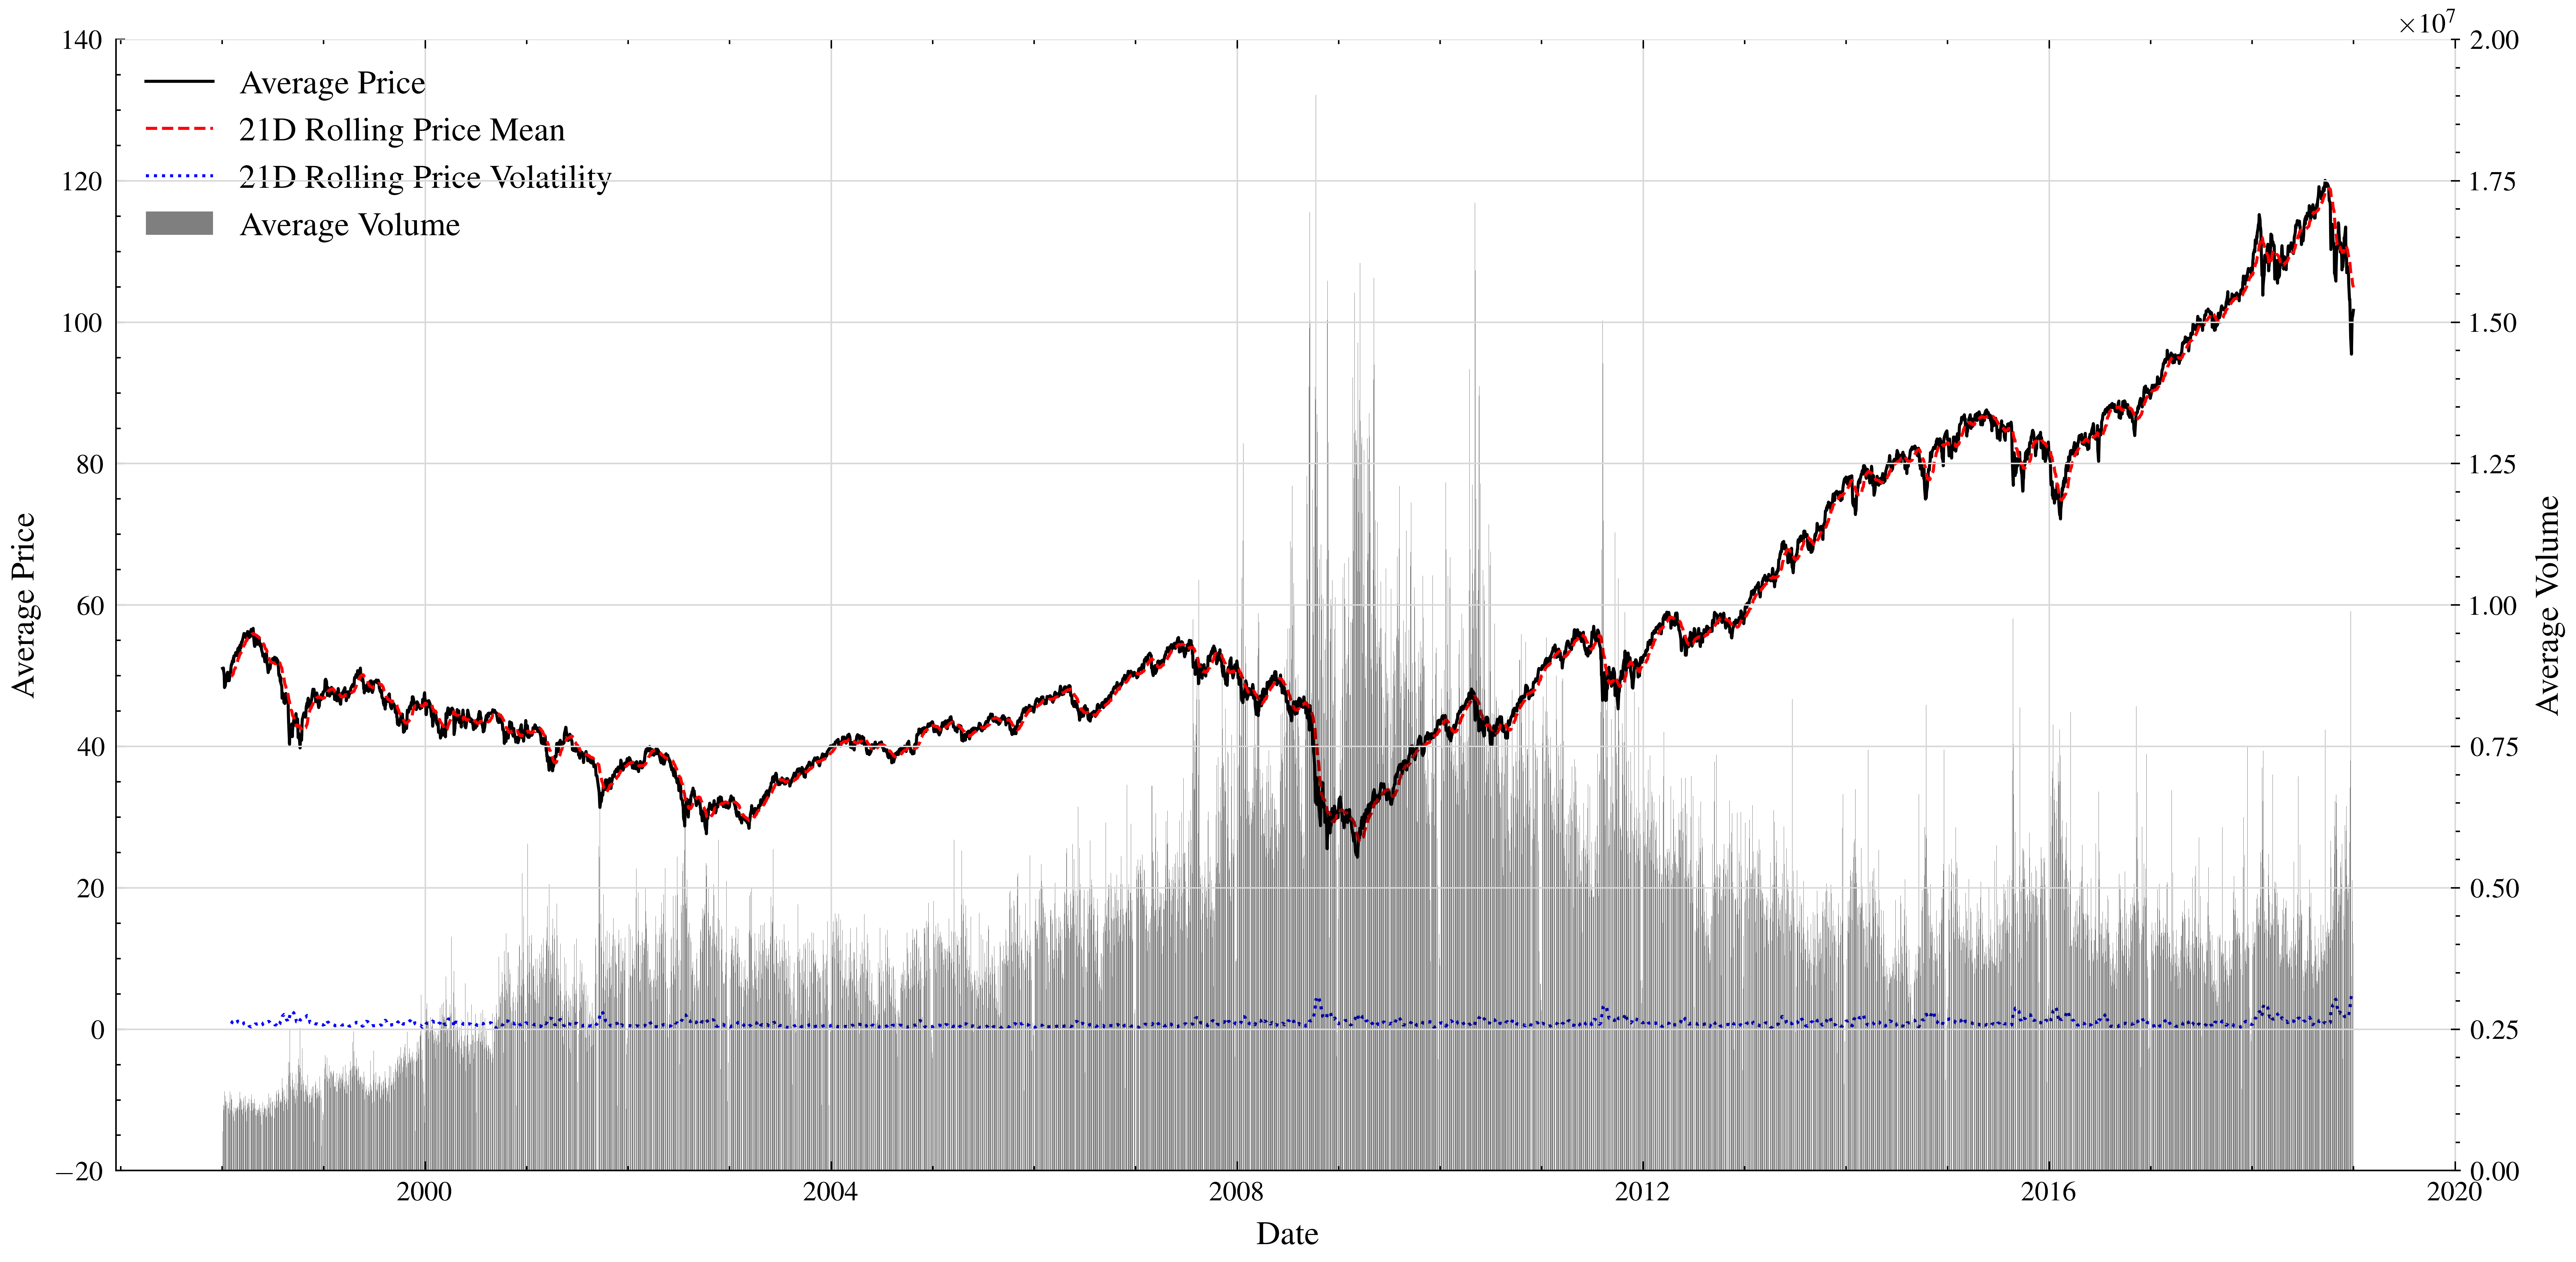
\includegraphics[width=\textwidth]{/Users/minhquangngo/Documents/vsc/erasmus/msc_thesis/latex/plots/data/summary_stats_avgprice_avgvol.png}
    \caption{Average price and volume in the sample period (1998-2018).}
    \label{fig:avgprice_avgvol}
\end{figure}

\begin{table}[H]
  \centering
  \caption{\textit{Descriptive Statistics (1/3)}}
  \label{tab:descr_stats}
  
  \begin{tabular}{lcccc}
  \toprule
  Statistic & $prc$ & $ret$ & $vol$ & $put\_call\_ratio$ \\\midrule
  N & 2646071 & 2645995 & 2646067 & 2631963 \\
  Mean & 56.690 & 0.000 & 4644742.786 & 2.451 \\
  SD & 70.228 & 0.025 & 14088422.298 & 35.811 \\
  Min & -116.812 & -0.942 & 0.000 & 0.000 \\
  Q1 & 27.660 & -0.010 & 915800.000 & 0.259 \\
  Median & 43.380 & 0.000 & 1987272.000 & 0.626 \\
  Q3 & 65.570 & 0.010 & 4372000.000 & 1.208 \\
  Max & 2206.090 & 1.024 & 1897900032.000 & 20979.000 \\
  \bottomrule
  \end{tabular}
  \end{table}
  
  \begin{table}[H]
  \centering
  \caption{Descriptive Statistics (2/3)}
  \label{tab:descr_stats2}
  
  \begin{tabular}{lcccccc}
  \toprule
  Statistic & $mktrf$ & $smb$ & $hml$ & $rmw$ & $umd$ & $cma$ \\\midrule
  N & 2646081 & 2646081 & 2646081 & 2646081 & 2646081 & 2646081 \\
  Mean & 0.000 & 0.000 & 0.000 & 0.000 & 0.000 & 0.000 \\
  SD & 0.012 & 0.006 & 0.007 & 0.005 & 0.010 & 0.004 \\
  Min & -0.089 & -0.042 & -0.044 & -0.030 & -0.082 & -0.059 \\
  Q1 & -0.005 & -0.003 & -0.003 & -0.002 & -0.004 & -0.002 \\
  Median & 0.001 & 0.000 & -0.000 & 0.000 & 0.001 & 0.000 \\
  Q3 & 0.006 & 0.004 & 0.003 & 0.003 & 0.005 & 0.002 \\
  Max & 0.114 & 0.045 & 0.049 & 0.045 & 0.071 & 0.025 \\
  \bottomrule
  \end{tabular}
  \end{table}
  
  \begin{table}[H]
  \centering
  \caption{Descriptive Statistics (3/3)}
  \label{tab:descr_stats3}
  
  \begin{tabular}{lccc}
  \toprule
  Statistic & $rf$ & $enhanced\_baker$ & $vix\_close$ \\\midrule
  N & 2646081 & 2646081 & 2645576 \\
  Mean & 0.000 & -0.264 & 20.197 \\
  SD & 0.000 & 2.023 & 8.497 \\
  Min & 0.000 & -5.085 & 9.140 \\
  Q1 & 0.000 & -1.567 & 13.870 \\
  Median & 0.000 & -0.287 & 18.530 \\
  Q3 & 0.000 & 0.980 & 24.030 \\
  Max & 0.000 & 5.254 & 80.860 \\
  \bottomrule
  \end{tabular}
  \end{table}
  
  

The late-2018 equity downturn was precipitated by escalating US-China trade tensions, as each new round of tariffs eroded investor confidence in global supply chains. Simultaneously, the Federal Reserve's fourth rate hike of the year and the brief inversion of the Treasury yield curve heightened recession fears among market participants. Signs of a synchronized global slowdown—particularly in Europe and emerging markets—further weighed on equity valuations as growth forecasts were revised downward. Finally, profit-taking in the technology sector, driven by concerns over maturing growth trajectories and mounting regulatory scrutiny, amplified the overall market sell-off \cite{reuters_2018}.

\begin{figure}[H]
     \centering
     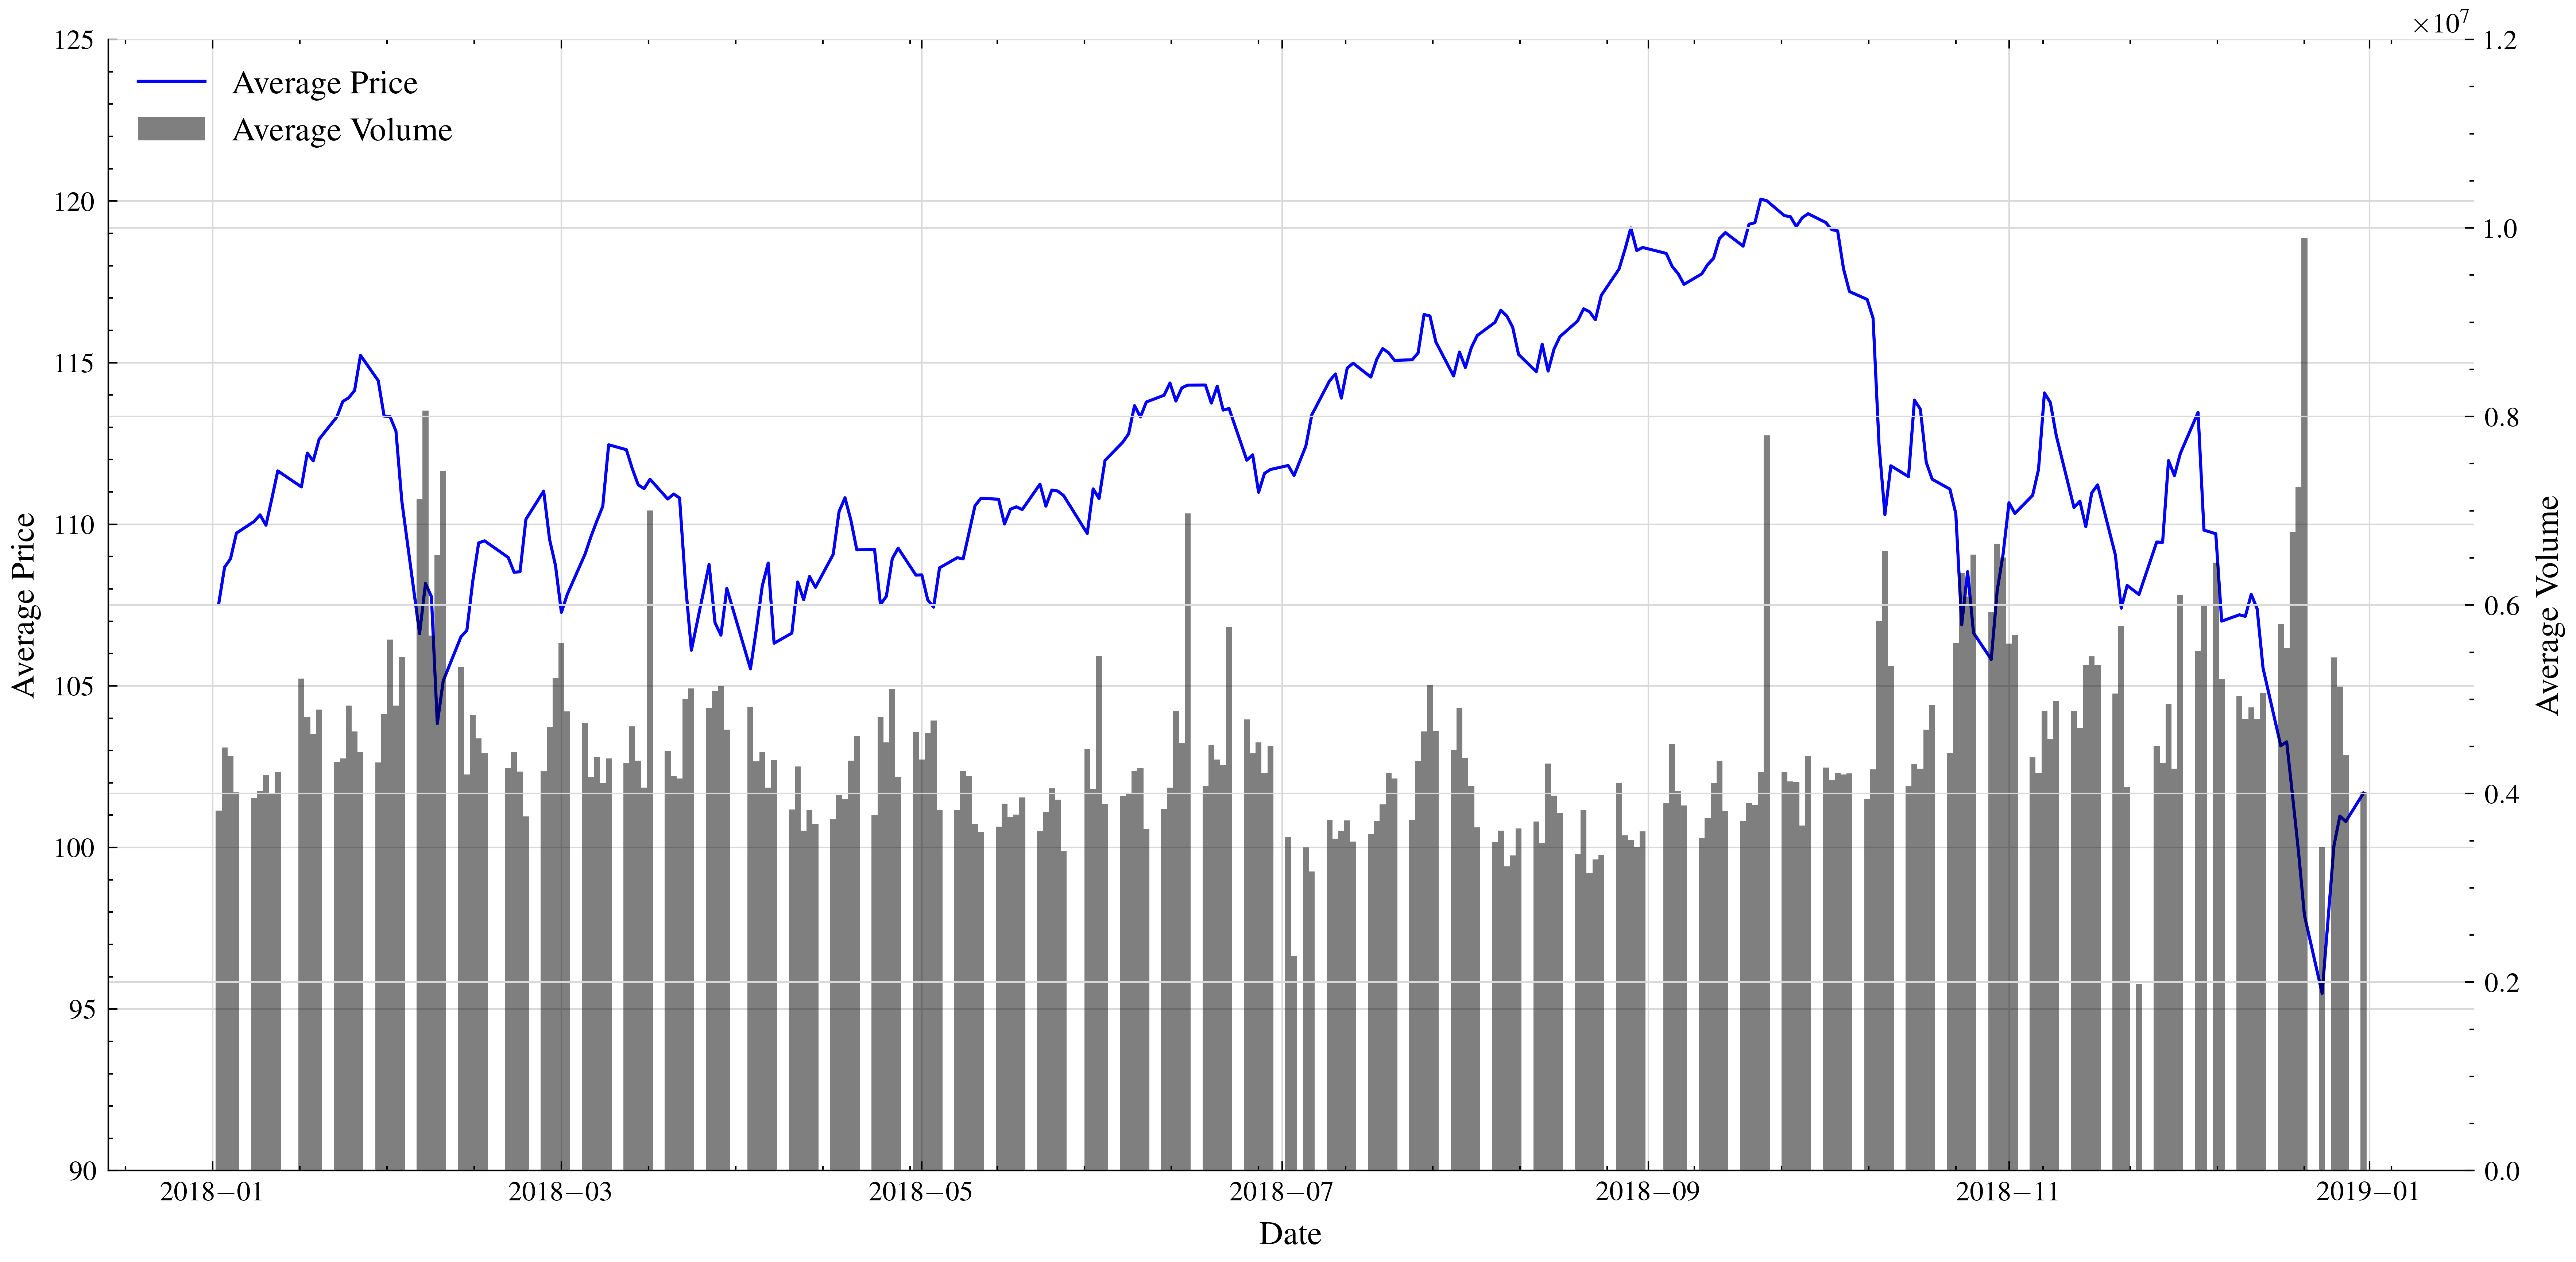
\includegraphics[width=\textwidth]{/Users/minhquangngo/Documents/vsc/erasmus/msc_thesis/latex/plots/data/summary_stats_avgprice_avgvol_2018.png}
     \caption{Average price and volume in the sample period (2018).}
     \label{fig:avgprice_avgvol_2018}
 \end{figure}

 \begin{table}[ht]
    \centering
    \caption{Descriptive Statistics 2018(1/3)}
    \label{tab:descr_stats_2018_1}
    
    \begin{tabular}{lcccccc}
    \toprule
    Statistic & $prc$ & $ret$ & $excess_ret$ & $vol$ & $baspread$ & $put_call_ratio$ \\\midrule
    N & 126228 & 126228 & 126228 & 126228 & 126228 & 126228 \\
    Mean & 111.667 & -0.000 & -0.000 & 4521230.109 & 2.509 & 2.007 \\
    SD & 150.655 & 0.018 & 0.018 & 9226770.951 & 4.228 & 39.952 \\
    Min & 2.630 & -0.418 & -0.418 & 64637.000 & 0.020 & 0.000 \\
    Q1 & 47.420 & -0.009 & -0.009 & 1179017.500 & 0.870 & 0.354 \\
    Median & 77.460 & 0.001 & 0.000 & 2225857.000 & 1.500 & 0.668 \\
    Q3 & 128.530 & 0.009 & 0.009 & 4526956.000 & 2.690 & 1.208 \\
    Max & 2206.090 & 0.454 & 0.454 & 344976676.000 & 170.738 & 12541.000 \\
    \bottomrule
    \end{tabular}
    \end{table}
    
    \begin{table}[ht]
    \centering
    \caption{Descriptive Statistics 2018(2/3)}
    \label{tab:descr_stats_2018_2}
    
    \begin{tabular}{lcccccc}
    \toprule
    Statistic & $mktrf$ & $smb$ & $hml$ & $rmw$ & $umd$ & $cma$ \\\midrule
    N & 126228 & 126228 & 126228 & 126228 & 126228 & 126228 \\
    Mean & -0.000 & -0.000 & -0.000 & -0.000 & 0.000 & 0.000 \\
    SD & 0.011 & 0.005 & 0.006 & 0.004 & 0.006 & 0.004 \\
    Min & -0.040 & -0.016 & -0.018 & -0.011 & -0.018 & -0.011 \\
    Q1 & -0.004 & -0.004 & -0.004 & -0.003 & -0.003 & -0.002 \\
    Median & 0.001 & -0.000 & -0.002 & 0.000 & 0.001 & -0.000 \\
    Q3 & 0.006 & 0.003 & 0.003 & 0.002 & 0.004 & 0.002 \\
    Max & 0.051 & 0.013 & 0.023 & 0.011 & 0.018 & 0.013 \\
    \bottomrule
    \end{tabular}
    \end{table}
    
    \begin{table}[ht]
    \centering
    \caption{Descriptive Statistics 2018(3/3)}
    \label{tab:descr_stats_2018_3}
    \begin{tabular}{lccc}
    \toprule
    Statistic & $rf$ & $enhanced_baker$ & $vix_close$ \\\midrule
    N & 126228 & 126228 & 126228 \\
    Mean & 0.000 & 1.258 & 16.605 \\
    SD & 0.000 & 1.171 & 5.059 \\
    Min & 0.000 & -1.372 & 9.150 \\
    Q1 & 0.000 & 0.659 & 12.640 \\
    Median & 0.000 & 1.577 & 15.430 \\
    Q3 & 0.000 & 2.103 & 19.890 \\
    Max & 0.000 & 2.707 & 37.320 \\
    \bottomrule
    \end{tabular}
    \end{table}
 
    \begin{figure}[H]
        \centering
        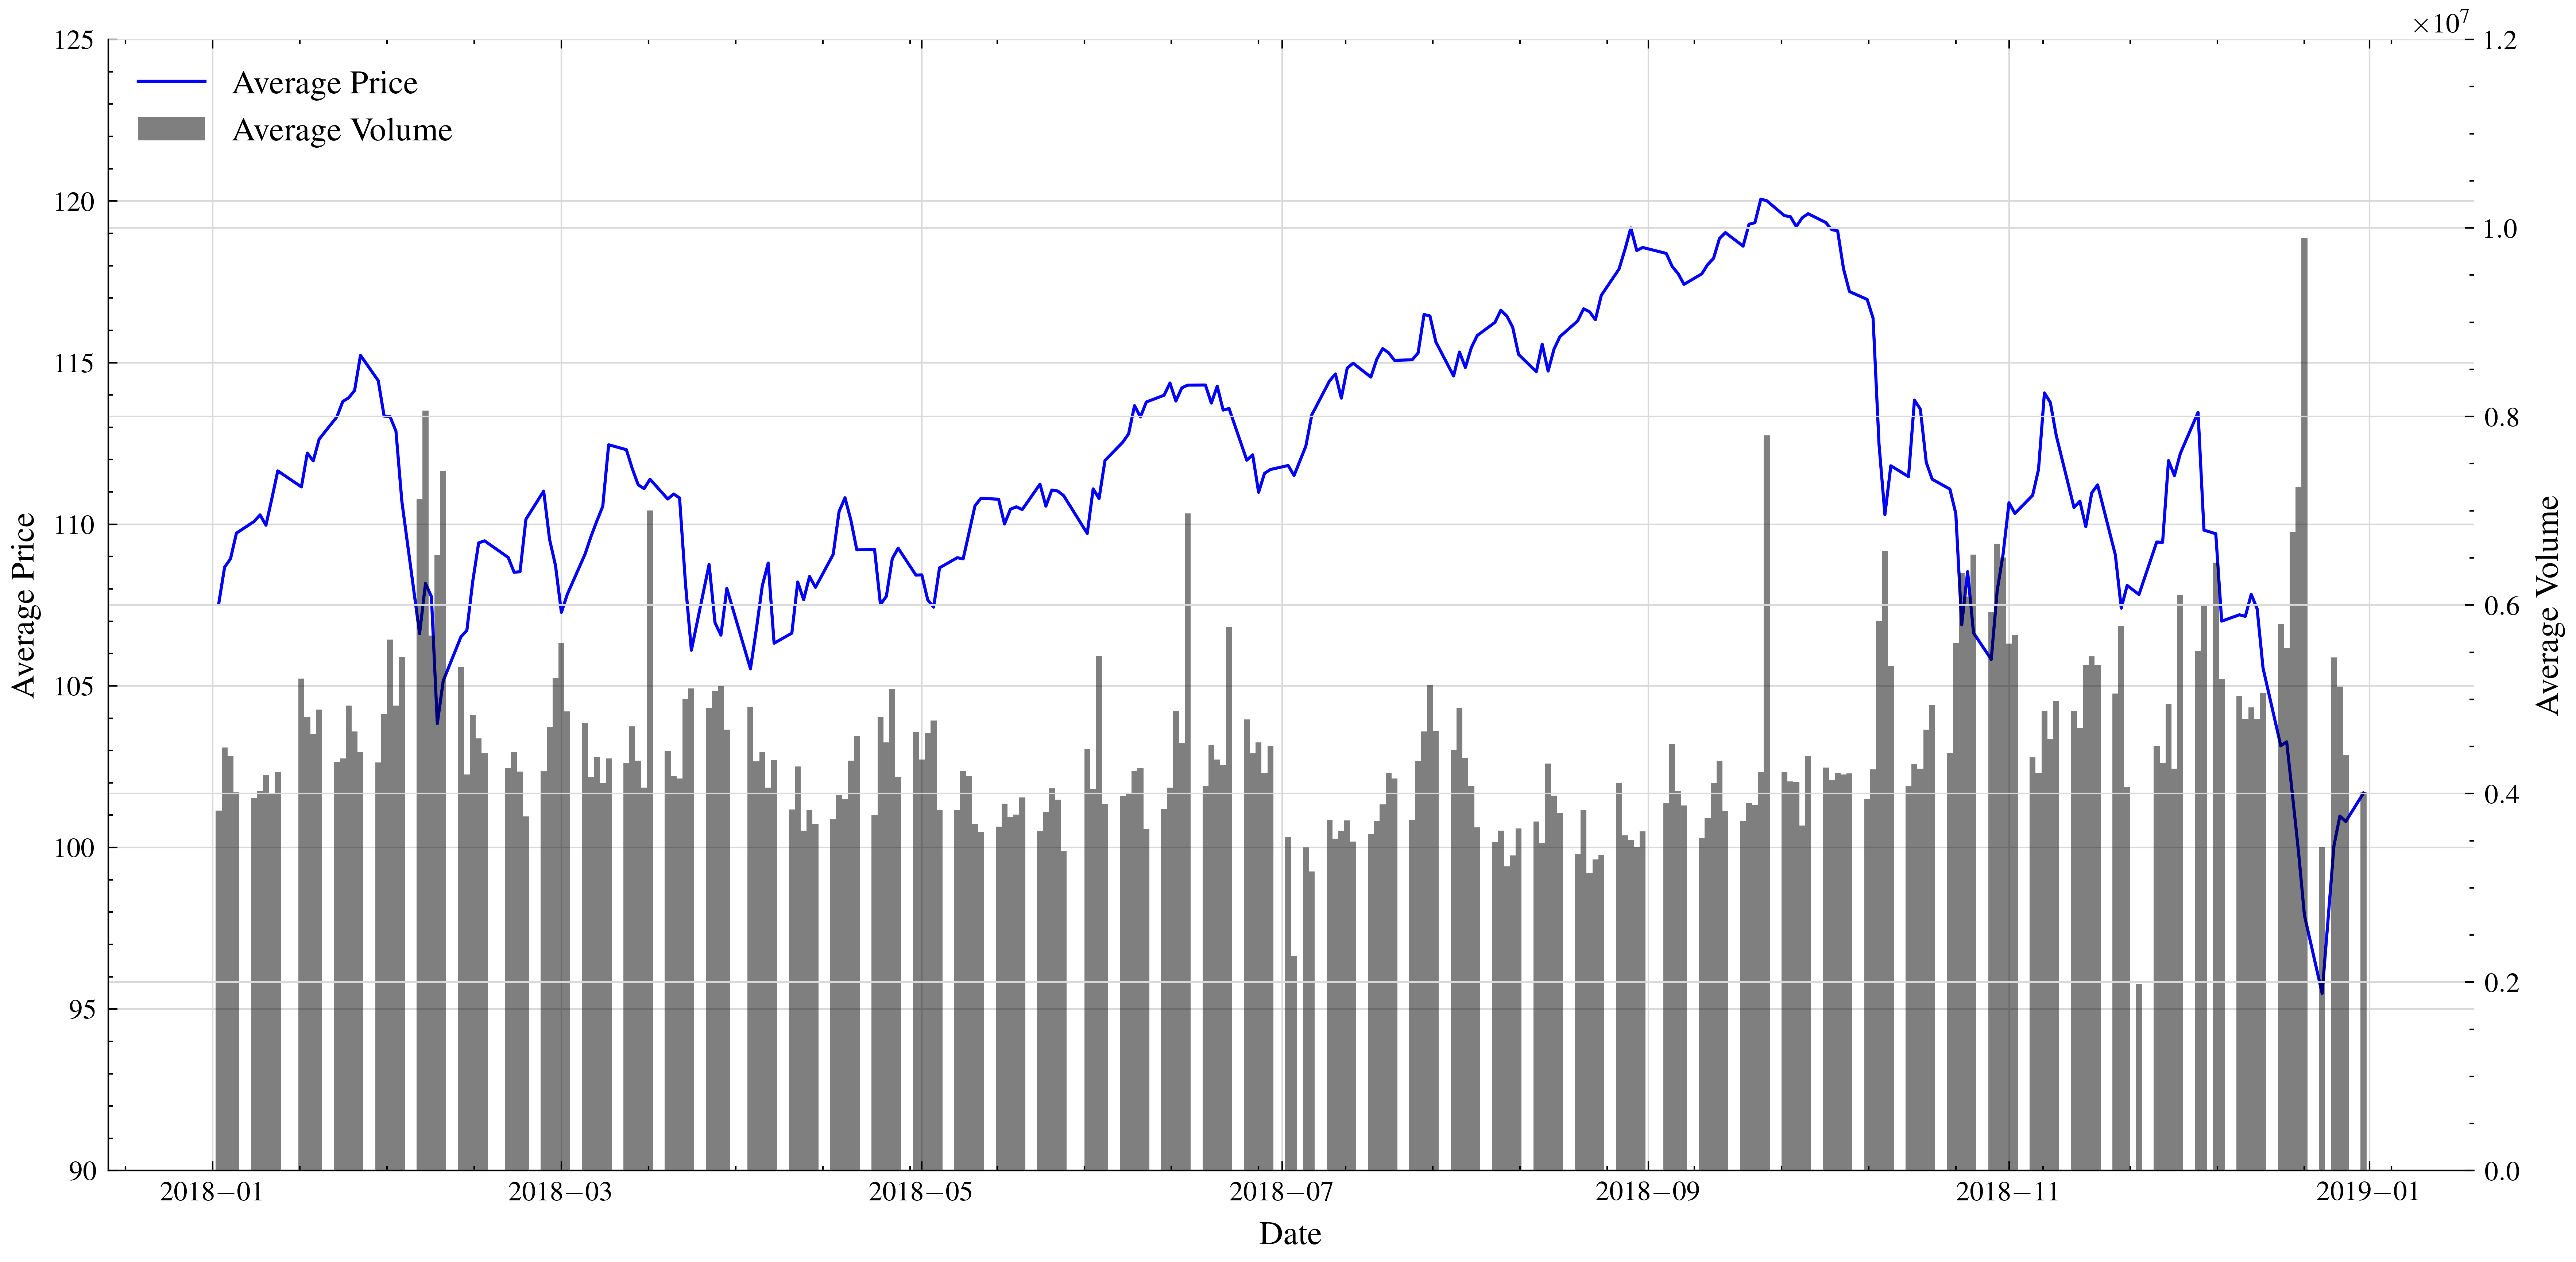
\includegraphics[width=\textwidth]{/Users/minhquangngo/Documents/vsc/erasmus/msc_thesis/latex/plots/data/summary_stats_avgprice_avgvol_2018.png}
        \caption{Average price and volume in the sample period (2018).}
        \label{fig:avgprice_avgvol_2018}
    \end{figure}

 Figure \ref{fig:his_mktrf_ret_rf} suggest that individual stock returns and broad market returns both oscillate around a constant mean of zero with roughly stable variance over time, indicating weak stationarity. Meanwhile, the risk-free rate appears as a near-point mass at zero, further confirming its stationary behavior given its negligible volatility. However, to formally verify stationarity we apply the Augmented Dickey-Fuller (ADF) test. It tests the null hypothesis that a time series contains a unit root (i.e.\ is non-stationary) against the alternative of stationarity. The resulting ADF statistic, done on a full panel OLS regression shows an ADF statistic of -30.6 with a p-value below 0.001, which decisively rejects the null, confirming that all three return series are stationary.


\begin{figure}[H]
     \centering
     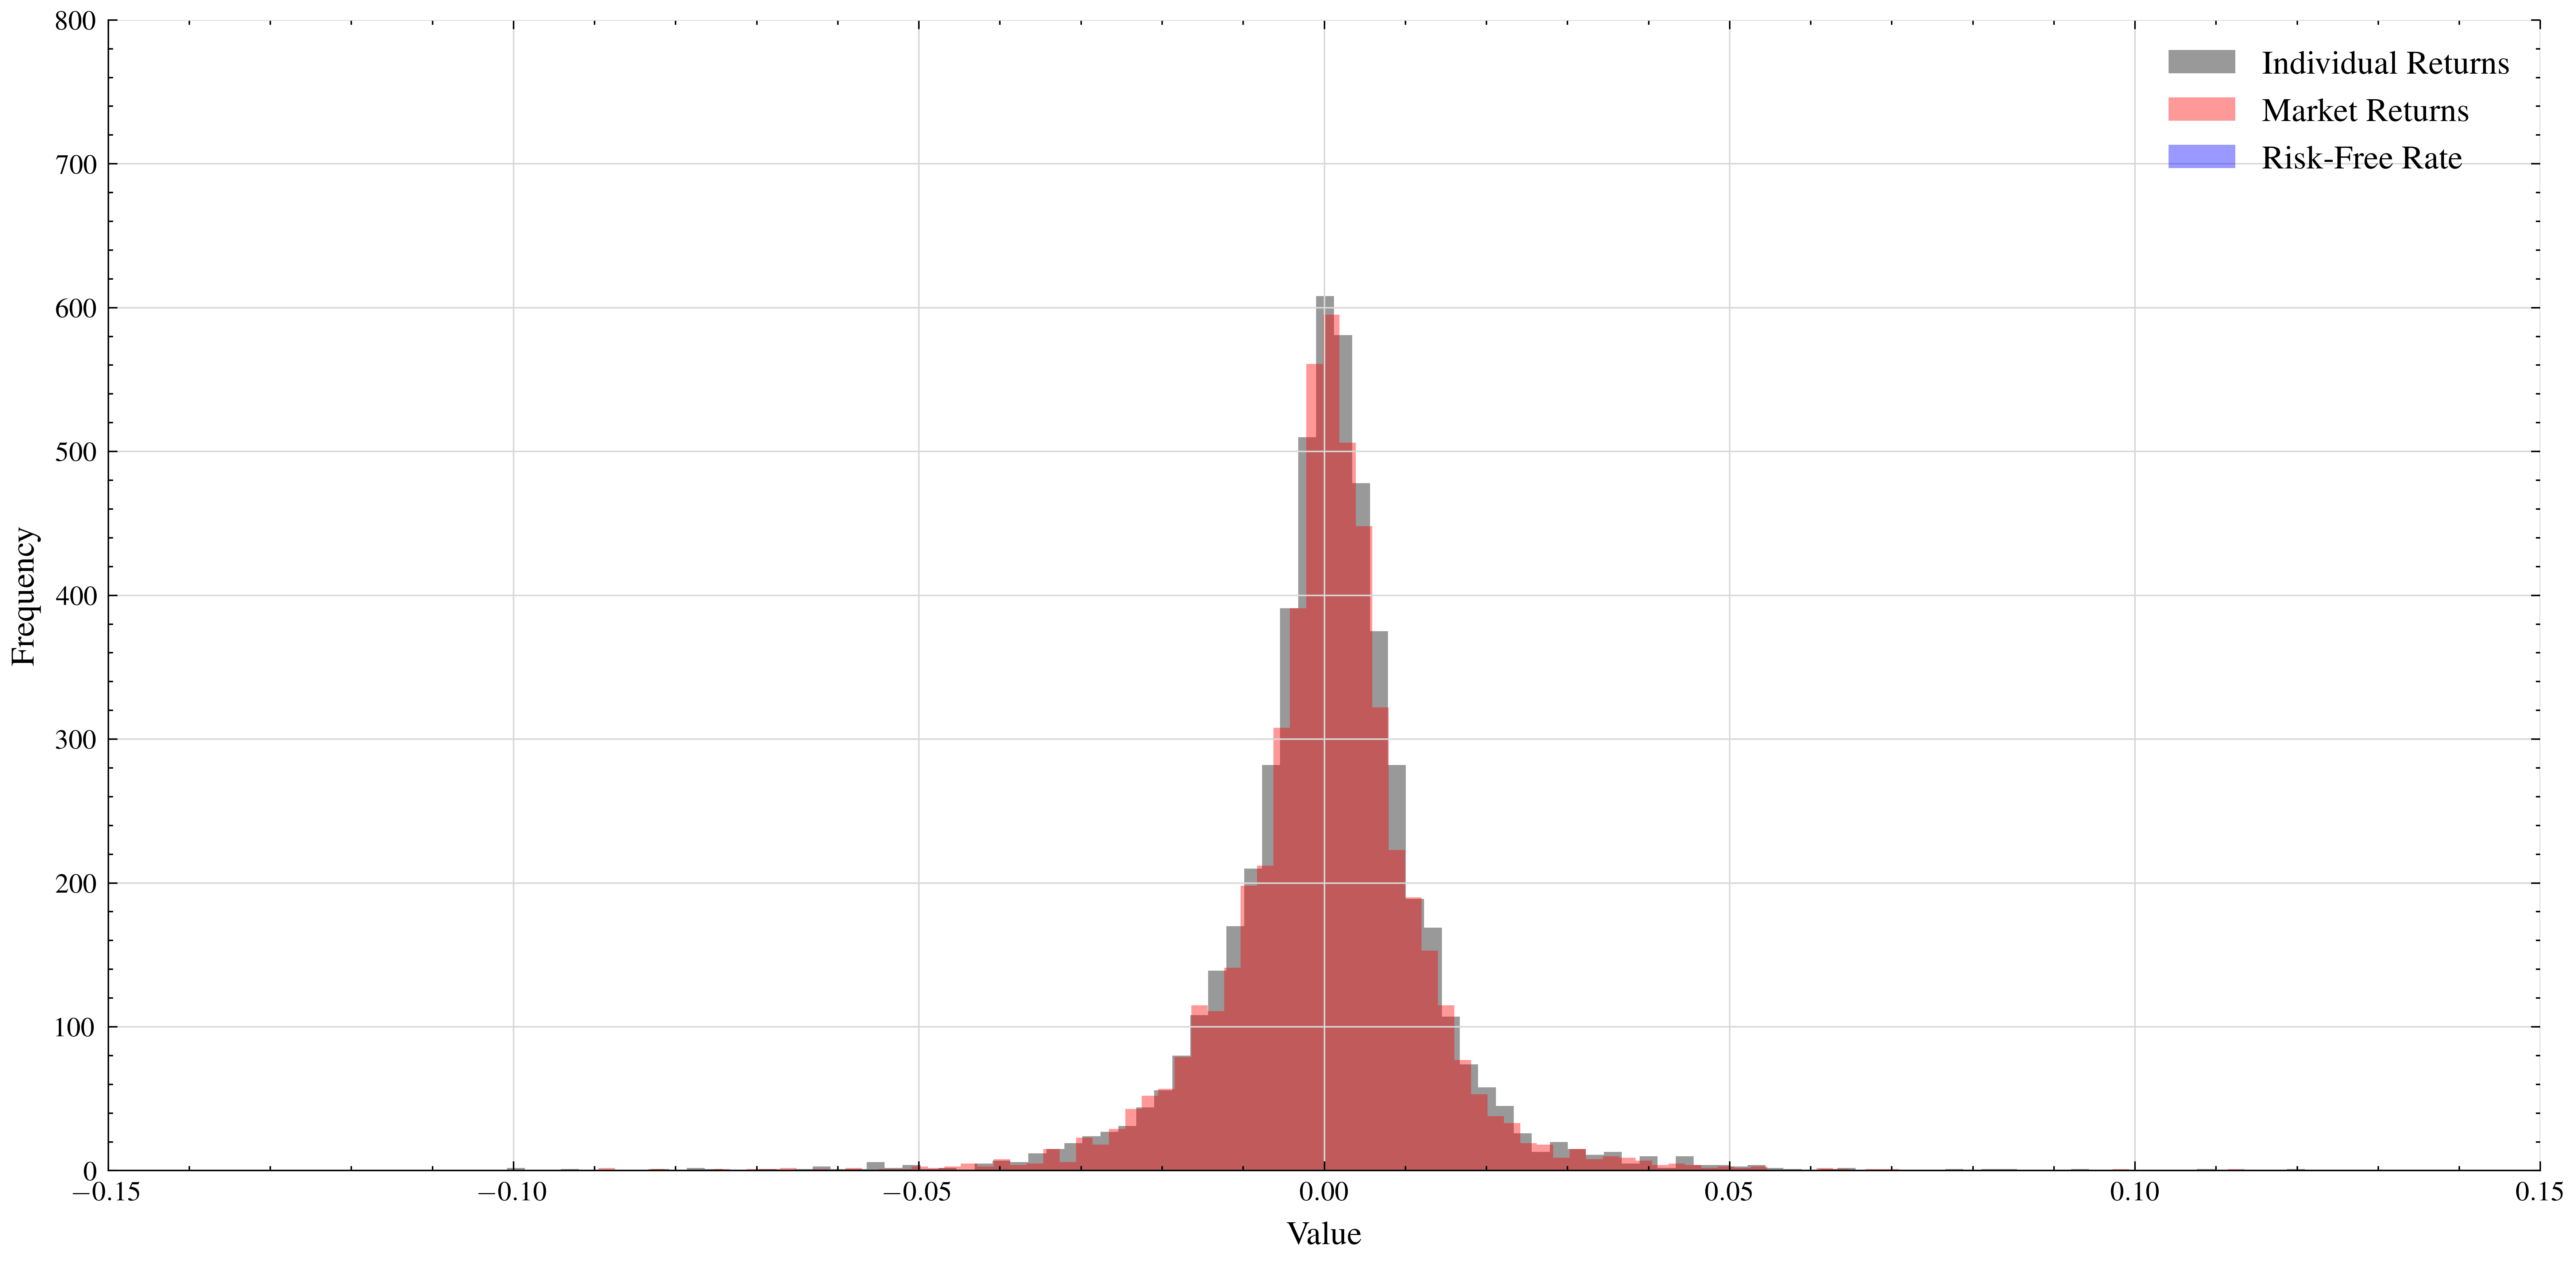
\includegraphics[width=\textwidth]{/Users/minhquangngo/Documents/vsc/erasmus/msc_thesis/latex/plots/data/hist_mktrf_ret_rf.png}
     \caption{Distribution of returns, factors, liquidity, sentiment.}
     \label{fig:his_mktrf_ret_rf}
 \end{figure}

 Variance inflation factors (VIFs) quantify the extent to which multicollinearity among regressors inflates the variance of estimated coefficients. They are defined as
 \begin{equation}
 \label{eq:vif}
\mathrm{VIF}_j = \frac{1}{1 - \beta_j^2},
\end{equation}

where $\beta_j^2$ is the coefficient of determination from regressing the $j$-th predictor on all other predictors.

 The VIFs in Table \ref{tab:vif} show that, while most predictors exhibit minimal collinearity (VIFs near 1), two liquidity measures stand out with markedly elevated values: turnover and dollar trading volume. Such high VIFs indicate that these variables are highly linearly related to other regressors, violating the OLS assumption that features are not multicollinear. In particular, a VIF above 10 for dollar volume suggests severe redundancy, which can inflate coefficient variances and undermine the stability of parameter estimates. By contrast, variables like SMB, HML and the Enhanced Sentiment Index maintain low VIFs (around 1), indicating they contribute largely unique information to the model. To address high multicollinearity for attribution, one could consider removing or combining one of these highly correlated liquidity proxies (e.g., via PCA or LASSO) to restore estimation precision. However, since the comparison criteria for this paper is based on the predictive power of the models, and the OLS serves as baseline, we will not explicitly address this issue.


 \begin{table}[H]
    \centering
    \caption{\textit{Variance inflation factors}}
    \label{tab:vif}
    % Resize to full text width so the wide table fits the page
    \resizebox{\textwidth}{!}{%
    \begin{tabular}{l*{15}{c}}
        \toprule
        excess\_mkt\_ret & smb & hml & umd & cma & turn & turn\_sd & mvel1 & dolvol & daily\_illq & zero\_trade\_ratio & baspread & enhanced\_baker & vix\_close & put\_call\_ratio & news\_sent \\
        \midrule
        1.264 & 1.024 & 1.598 & 1.310 & 1.548 & 10.613 & 2.019e-17 & 2.497 & 13.034 & 1.875 & 1.042 & 2.647 & 1.114 & 2.428 & 1.021 & 1.994 \\
        \bottomrule
    \end{tabular}}
\end{table}

Figure~\ref{fig:sector_price} shows that most sectors move in tandem at modest levels until roughly 2005, after which dispersion (and thus opportunities for investors) begins to emerge. The full list of descriptive statistics for each sector is provided in the appendix, with \cref{sec:descriptive_statistics}. With 11 sectors, there are some data points for these sectors that are worth noting. Notably, the Real Estate sector (60) surges from a roughly \$50 baseline to nearly \$900 by 2018-19, far outstripping its peers. The sector's rapid ascent (after the 2008 financial crisis) mark it as a high-beta, high-reward investment. The sector exhibits an average daily return of 0.001\% alongside substantial daily volatility of 0.02\%, 100\% higher than on average. With mean daily dollar trading volume near \$13.5 million and turnover spiking to 50 \% on certain days, this market remains exceptionally active and had exceptional performance due to several macroeconomic factors. After the 2008 crash, central banks drove interest rates down to almost zero and bought massive amounts of bonds, which made real estate look like a much better deal than savings or government debt. Big pension funds and insurance companies, desperate for higher returns, poured billions into property markets, pushing prices up even further. In many major cities, tough zoning laws and a shortage of new construction meant there simply were not enough homes or offices to go around, so prices climbed rapidly. At the same time, wealthy investors from all over the world snapped up trophy buildings and luxury developments, driving the Real Estate sector index up \cite{cbre_2018}. %VOLUME/TURNOVER

%THERE ARE ROOM TO IMPROVE THIS. MAYBE 2nd DRAFT
The Communication Service (50) sector demonstrates significant volatility, with pronounced drawdowns around the end of 2009 and a massive plunge in mid-2014. These sharp reversals highlight the sector's sensitivity to both macroeconomic shocks and industry-specific disruptions, yet its underlying growth drivers support a rapid recovery. Even after the 2008 crisis, this sector saw an immediate rebound. By the late 2010s, Communication Services had rebounded steadily to rank among the priciest investment sectors, showing that this sector has a strong appeal despite intermittent bouts of extreme risk.Information Technology (45) staged a dramatic recovery after the 2008-09 financial crisis, surging from its troughs into sustained rapid growth. However, this ascent was interrupted by a sharp correction in early 2013 and an even more pronounced plunge in 2015. Although the sector began closing the gap on its pre-plunge highs by 2018, the pace of recovery implies that, if current trends persist, it may take several more years before Information Technology fully retraces its earlier losses.

%SECTOR 45


\begin{figure}[H]
     \centering
     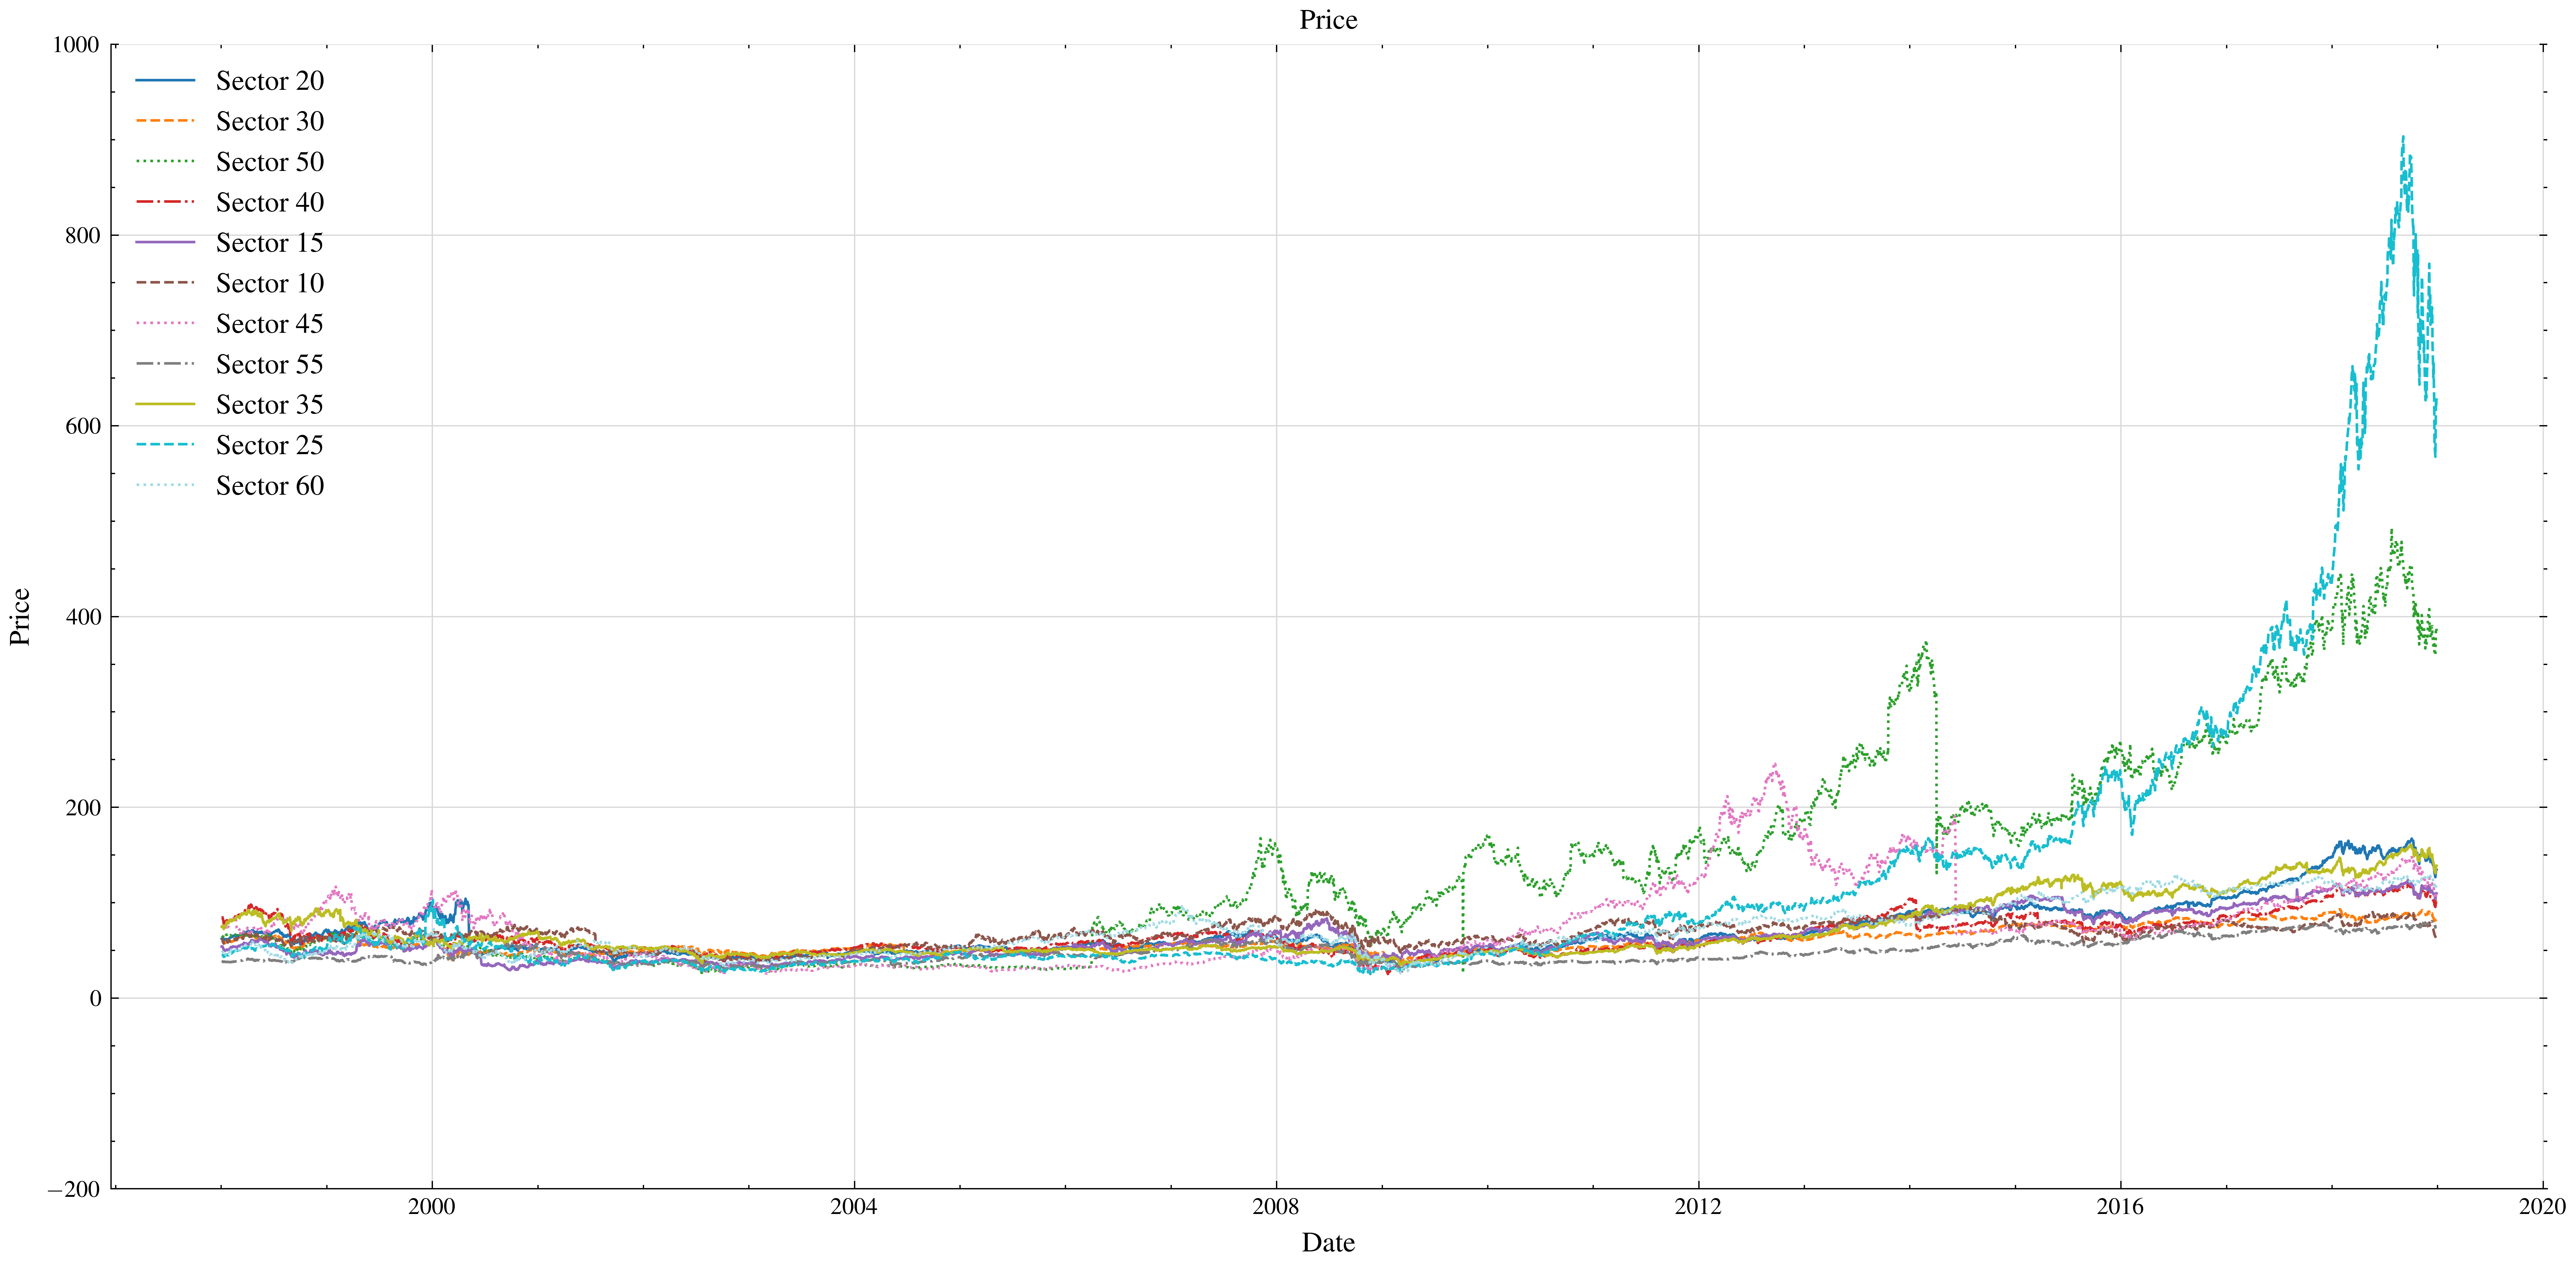
\includegraphics[width=\textwidth]{plots/data/sector_price.png}
     \caption{Sector price (1998--2018)}\label{fig:sector_price}
 \end{figure}


 

% 4.6 Descriptive Statistics and Preliminary Visualizations
%   4.6.1 Summary statistics for all variables (mean, SD, skew, kurtosis)
%   Table 4.3: Descriptive statistics of returns, factors, liquidity, sentiment
%   4.6.2 Histograms of ILLQ, turnover, sentiment index—assess distributional shape
%   Figure 4.1: Histogram grid of liquidity proxies and STV
%   4.6.3 Time‐series plots of aggregate liquidity and sentiment indices (1990–2018)
%   Figure 4.2: Overlay of monthly Amihud ILLQ and STV series
%   4.6.4 Cross‐variable correlation heatmap (factors vs. liquidity vs. sentiment)
%   Figure 4.3: Correlation matrix heatmap



